\begin{figure}[t]
    \centering
        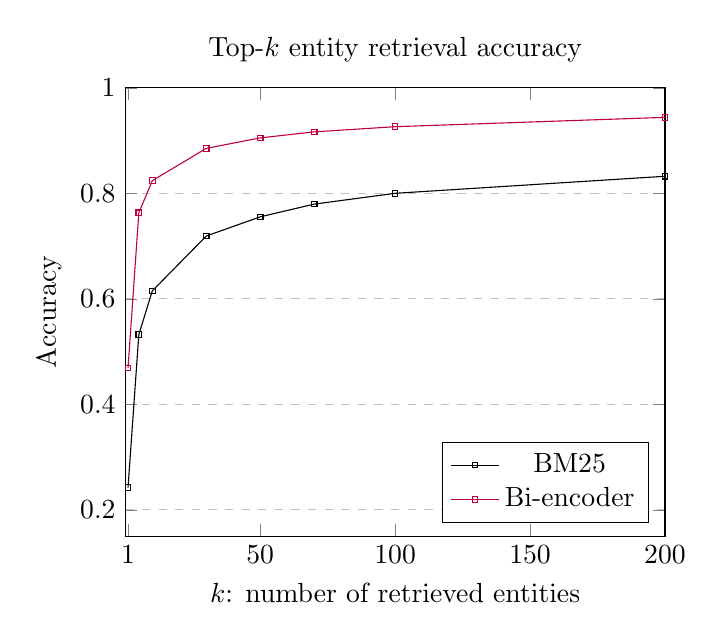
\begin{tikzpicture}
        \begin{axis}[
            title={Top-$k$ entity retrieval accuracy},
            xlabel={$k$: number of retrieved entities},
            ylabel={Accuracy},
            xmin=0, xmax=200,
            ymin=0.15, ymax=1,
            xtick={1,50,100,150,200},
            ytick={0,0.2,0.4,0.6,0.8,1},
            legend pos=south east,
            ymajorgrids=true,
            grid style=dashed,
        ]
         
        \addplot[
            color=black,
            mark=square,
            mark size=1pt
            ]
            coordinates {
            (1, 0.2422)(5, 0.5322)(10, 0.6151)(30, 0.7191)(50, 0.7555)(70, 0.7796)(100, 0.8001)(200, 0.8324)(300, 0.8498)(400, 0.8596)(500, 0.8651)
            };
            \addlegendentry{BM25}

        \addplot[
            color=purple,
            mark=square,
            mark size=1pt
            ]
            coordinates {
            (1,0.4689)(5,0.7631)(10,0.8240)(30,0.8853)(50,0.9052)(70,0.9166)(100,0.9264)(200,0.9441)(300,0.9530) (400,0.9580) (500,0.9617)
            };
            \addlegendentry{Bi-encoder}


        \end{axis}
        \end{tikzpicture}
    \caption{Top-$k$ entity retrieval accuracy on validation dataset of Zero-shot EL dataset}
    \label{fig:retrieval}
\end{figure}
